\scanpage{61}
Partant des MD-graphes ``élémentaires'' correspondants, je voudrais expliciter dans les quatre cas la structure \inserted{de spécialisation entre} des strates des $\widehat M_{g,\nu}$ et $\widehat M^!_{g,\nu}$.

8) \uline{Structure de spécialisation des strates en dim modulaire $\leq2$.}

$1^\circ)$ \uline{Cas \unsure{de|des}} $\widehat M^!_{0,4}$ \uline{et} $\widehat M_{0,4}$

Commençons par $\widehat M^!_{0,4}$.
\figure{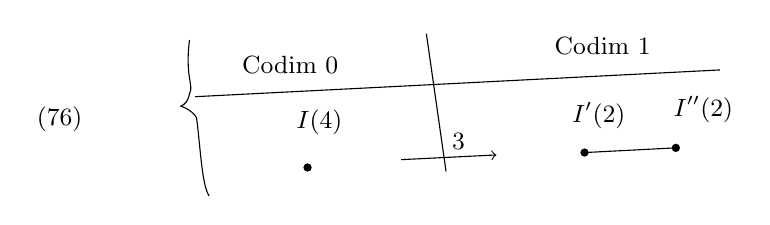
\begin{tikzpicture}[x=.010cm,y=-.010cm,every node/.style={font=\small}]
\node at (-183,33) {$(76)$};
\draw (-18,-68) .. controls (-24,-20) and (-12,-10) .. (-18,0) .. controls (-20,10) and (-23,13) .. (-29,16) .. controls (-17,20) and (-10,28) .. (-9,31) .. controls (-4,70) and (-2,118) .. (7,130);
\draw (-11,4)--(656,-30);\draw (283,-76)--(308,99);
\node at (110,-36) {Codim $0$};\node at (507,-61) {Codim $1$};
\node at (147,36) {$I(4)$};\fill (132,94) circle(1.5pt);
\draw[->] (251,84)--(372,78);\node at (324,61) {$3$};
\node at (502,28) {$I'(2)$};\node at (635,20) {$I''(2)$};
\draw (484,75)--(600,69);\fill (484,75) circle(1.5pt);\fill (600,69) circle(1.5pt);
\end{tikzpicture}}
Le diagramme signifie que l'ens. marqué $I$ de cardinal $4$, \inserted{\unsure{se partageant|se partage}} suivant l'une quelc. des trois partitions de $I$ en $I'$ et $I''$ de cardinal $2$ chacun, donne $3$ spécialisations différentes de la strate \unsure{maxima|maxim.} --- cela correspond bien sûr aux trois pts à l'infini de $U_{0,3}$

on aura
\[
(77)\qquad \widehat M^!_{0,4}\simeq\mathbb P^1_{\mathbb Z},\quad M^!_{0,4}\simeq(U_{0,3})_{\mathbb Z}=\mathbb P^1_{\mathbb Z}\smallsetminus\{0,1,\infty\}
\]
Pour bien faire, il faudrait aussi expliciter
\margin{60}
